\chapter{Revisión de literatura}

\noindent Este capítulo está dividido en dos secciones.  

\newpage

\section{Modelos teóricos}

\subsection{Hechos estilizados}


% La siguiente gráfica está hecha a mano porque la que arroja R se pixelea un poco al importarla a LaTeX. Pueden apoyarse en Excel para obtener las coordenadas más rápido

\begin{figure}[H]
\begin{center}
\caption{PIB mundial de los últimos dos milenios}
\label{PIB_MUN}
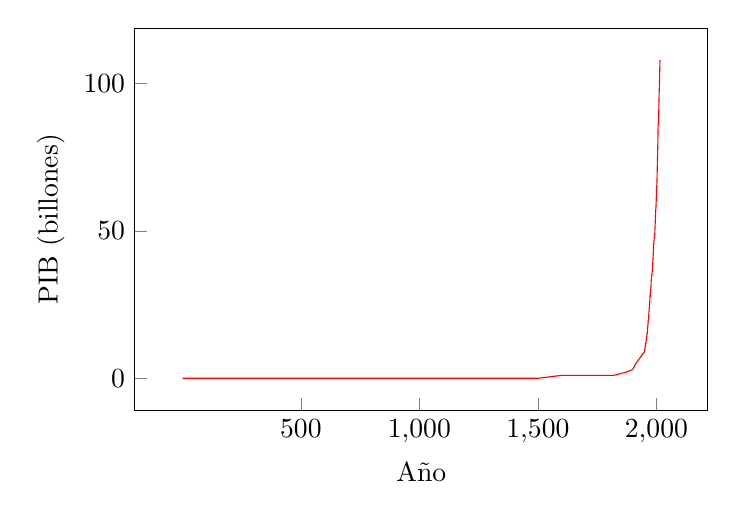
\begin{tikzpicture}
\begin{axis}[
    xlabel={Año},
    ylabel={PIB (billones)},
    xtick pos=left,
    ytick pos=left,
    xtick={500,1000,1500,2000},
    ytick={0,50,100},
    scale only axis=true,
    width=0.6\textwidth,
    height=0.4\textwidth,
]
 
\addplot[
    color=red,
    ]
    coordinates {
    (1,0)(1000,0)(1500,0)(1600,1)(1700,1)(1820,1)(1870,2)(1900,3)(1913,5)(1940,8)(1950,9)(1951,10)(1952,10)(1953,11)(1954,11)(1955,12)(1956,12)(1957,13)(1958,13)(1959,14)(1960,15)(1961,15)(1962,16)(1963,17)(1964,18)(1965,19)(1966,20)(1967,20)(1968,22)(1969,23)(1970,24)(1971,25)(1972,26)(1973,28)(1974,28)(1975,29)(1976,30)(1977,31)(1978,33)(1979,34)(1980,35)(1981,35)(1982,36)(1983,37)(1984,38)(1985,40)(1986,41)(1987,43)(1988,45)(1989,46)(1990,47)(1991,48)(1992,48)(1993,49)(1994,51)(1995,53)(1996,55)(1997,57)(1998,58)(1999,60)(2000,63)(2001,65)(2002,66)(2003,69)(2004,73)(2005,76)(2006,80)(2007,85)(2008,87)(2009,87)(2010,91)(2011,95)(2012,98)(2013,101)(2014,105)(2015,108)
    };
    
\end{axis}
\end{tikzpicture}

\imagesource{elaboración propia con datos de Maddison (2010) y el Banco Mundial.}
\end{center}
\end{figure}
